\chapter{Introduction}
\label{chapter:intro}

Distributed computing is used in a wide variety of areas
such as telecommunication, data processing, process control in real-time systems, etc~\cite{Lynch1996}. Similar to
how traditional algorithms are studied with a classical
centralized computational entity in mind, distributed
algorithms are developed to be used in distributed
systems that are becoming more and more ubiquitous in the
field of technology~\cite{Attiya2004}. Such distributed
systems consist of many computational units each
performing local computation and communicating
with other such units close to it. Figure~\ref{fig:classical-vs-distributed-computing} demonstrates
the difference between the centralized and distributed perspectives.

Unlike traditional
centralized algorithms, in distributed computing,
there is no centralized entity that would see the
entirety of the system's input or output. Instead,
input is shared among the computational units, each
knowing only a part of it. Also, once a distributed
algorithm halts, each unit is only aware of its
own output piece. This, among other things, implies
that it is now non-trivial to ensure that the
executed algorithm has succeeded and the
outputs of the computational units are
indeed valid when considered together.

\begin{figure}
  \centering
  \begin{subfigure}[b]{0.49\textwidth}
      \centering
      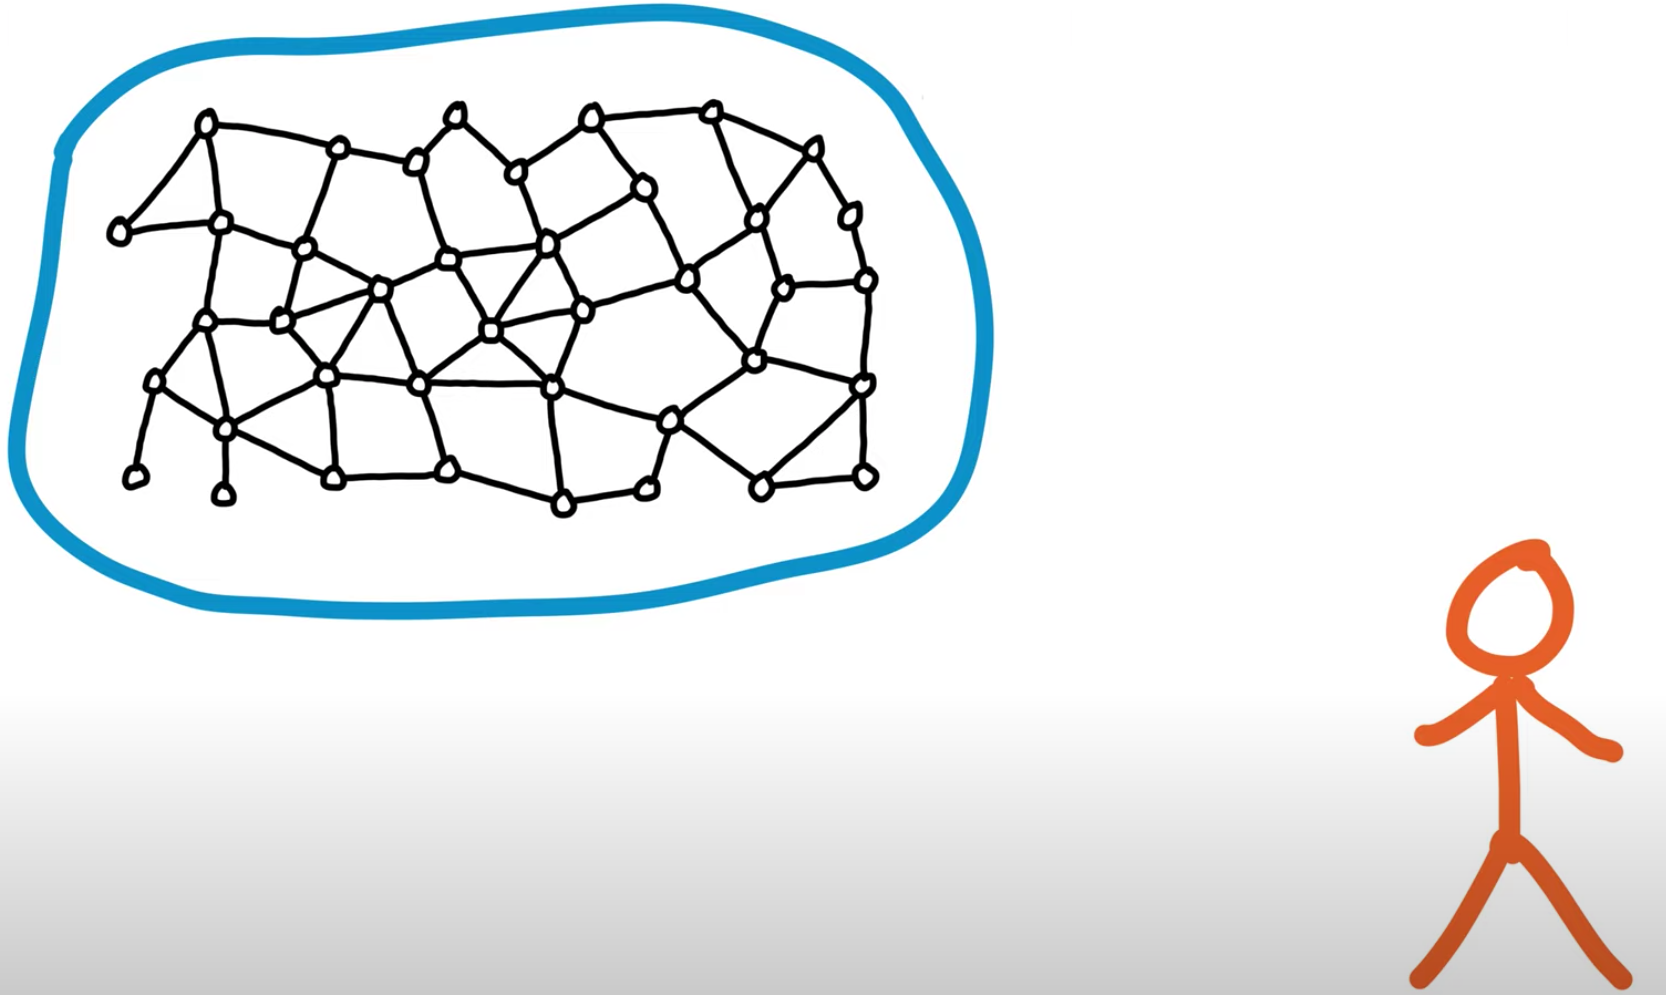
\includegraphics[width=\textwidth]{images/classical-computing.png}
      \caption{Perspective in classical computing}
      \label{fig:classical-computing}
  \end{subfigure}
  \hfill
  \begin{subfigure}[b]{0.49\textwidth}
      \centering
      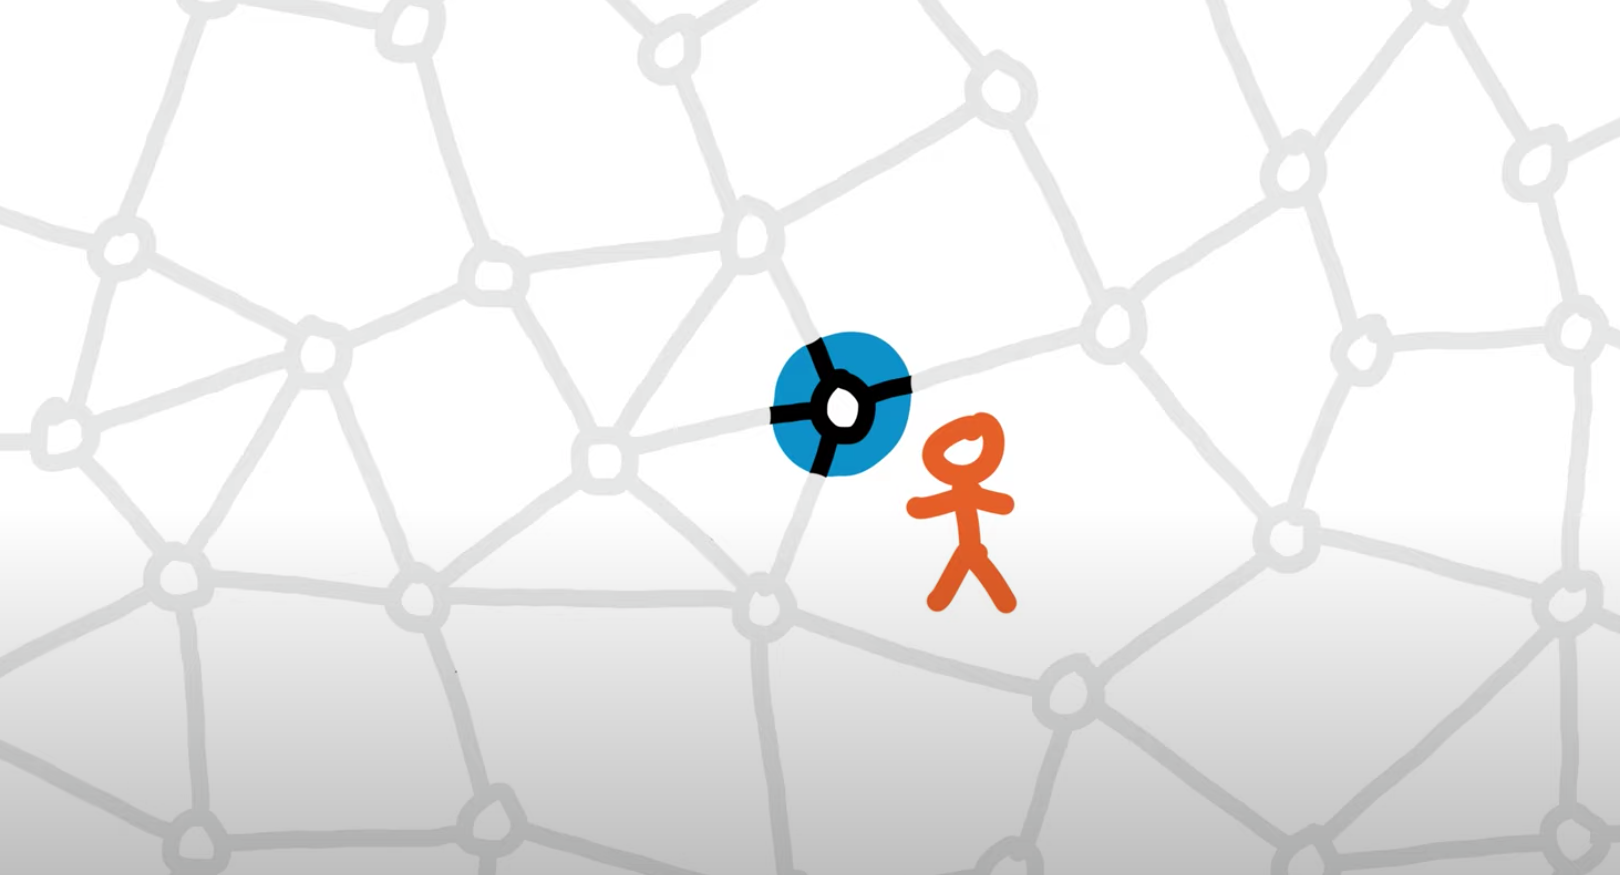
\includegraphics[width=\textwidth]{images/distributed-computing.png}
      \caption{Perspective in distributed computing}
      \label{fig:three sin x}
  \end{subfigure}
  \caption{
    The difference in perspectives in classical and distributed computing\protect\footnotemark.
    In the classical setting, a single all-seeing entity is given the whole graph,
    it solves a problem on the whole graph, and outputs the entire solution.
    In the distributed setting, there is no all-seeing entity. Instead, each node
    in the graph is performing some local computation, based on which each node
    produces only a part of the solution. The outputs of all the nodes are then combined
    to obtain the entire solution.
  }
  \label{fig:classical-vs-distributed-computing}
\end{figure}

The field of distributed algorithms has several
decades of research history and has grown
significantly since its inception in the 1980s.
One specific
area of the field that has received a lot of
attention in recent years from the scientific
community is the study of \emph{locally verifiable}
problems.
These are the kinds of problems, where, roughly speaking,
once execution of an algorithm has ended, each
computational unit can
collect information only from close-by computational units,
and it will be sufficient to ensure that the executed algorithm has succeeded. Problems of this kind are particularly
interesting because they have obvious relevance
in cases where the size of the network is extremely
large, and thus each computational unit
cannot afford to check every other unit in the system.

As the field has been studied, more and more knowledge
about such problems has been accumulated by the
research community. In particular, as is common
in the field of algorithm design, much of the
research has been focused on the complexity of
problems in distributed computing. Apart from
individual complexity results, the research
community has invented several \emph{meta-algorithms}.
These are centralized algorithms that
automatically determine the\footnotetext{The image was copied from the video~\cite{DA2020Introduction} that was a part of Distributed Algorithms 2020 course at Aalto University with the permission of the authors.}
computational complexity of a provided
problem.

\section{Problem statement}

The individual complexity results and the meta-algorithms
that determine the complexity of a specified problem are
scattered across tens of published papers. Each of the
papers uses a different problem representation and
formalism. This causes researchers to solve
the same problems again and again since no
centralized place exists that would accumulate all of the
above-mentioned results.

I will attempt to rectify the
problem by designing and implementing a system
that would allow researchers to quickly
access complexity-related results for locally
verifiable problems, provided such problems have been
already studied
previously. I expect that such a solution
would be of high value to the research community and
would save significant time resources, allowing the researchers
to concentrate on discovering new knowledge about the
field instead of spending time on solving problems that
have already been solved numerous times before.

\section{Structure of the thesis}
\label{section:structure} 

Chapter~\ref{chapter:background} provides a theoretical
background necessary for understanding the contents of the
following chapters. The chapter opens with
a brief but informative overview of graph-theoretic
concepts. Then, the chapter provides basic
theoretical background related to distributed computing.
Moreover, the chapter explains notions of
locally checkable labeling problems, decidability, as well as
covers recent developments in the area of
automated classification in distributed algorithms.

Chapter~\ref{chapter:environment} describes
meta-algorithms that are used in my final
solution. The meta-algorithms take a description
of a locally verifiable problem as an input and
as an output produce some information about the
problem's complexity.

Chapter~\ref{chapter:methods} states my research goals
and defines the scope of the thesis project.
Chapter~\ref{chapter:implementation}
provides an overview of an implementation of
my solution. Chapter~\ref{chapter:evaluation}
evaluates the outcomes of the implementation
against the earlier stated research goals. It
also points out possible directions for
future development. Finally, Chapter~\ref{chapter:conclusions}
summarizes the entirety of the work.
